

You will no doubt have heard of the concept of a ``small world'', where people measure the ``degree of proximity'' to a well-known person. 
For example, I know someone (A) who knows someone (B) who knows the Prime Minister:
\begin{itemize}
	\item Me $\to$ A $\to$ B $\to$ Prime Minister;
	\item This places me at 3 degrees from the Prime Minister.
\end{itemize}



\href{https://www.wikipedia.org/wiki/Paul_Erdos}{\emph{Paul Erd{\"o}s}} (1913-1996), was one of the most prolific mathematicians: yes, he published a lot (more than 1500 scientific articles), but he is also known to be an \emph{``original''}: he had no fixed home, always moved from place to place to work with friends. 
This very special life led to the creation of the \href{https://www.wikipedia.org/wiki/Erdos_number}{\emph{Erd{\"o}s number}} which works exactly like the degree of proximity to the Prime Minister or to any known person! 

\begin{emphbox}[]
In fact a whole website -- \url{https://oakland.edu/enp} -- is devoted to the work of Erd{\"o}s and his collaborators. On this site, we were able to extract a \textbf{\color{Green}database} $\bigg($\url{https://uoft.me/erdos} \qrcode[height=.35in]{https://uoft.me/erdos}$\ \bigg)$ which contains the list of mathematicians who have an Erd{\"o}s number $= 1$. 
Each line of this database contains:
\begin{itemize}
	\item $\big\{$number of collaborator (classified in alphabetical order),
	\item number of collaborators in this same list,
	\item number of collaborators who have a Erd{\"o}s number $= 2$,
	\item name of the mathematician, 
	\item number of collaborators in this list separated by a comma $\big\}$
\end{itemize}
\end{emphbox}

\begin{example}
\hfil \{1, 7, 16, "ABBOTT, HARVEY, LESLIE", 186, 308, 318, 321, 401, 429, 450\}

means that Harvey Abbott (no. 1 on this list) wrote papers with 7 others mathematicians whose Erd{\"o}s number is 1, and 16 whose Erd{\"o}s number is 2. His collaborators with Erd{\"o}s number $= 1$ bear the labels: 186, 308, 318, 321, 401, 429, 450. 
\end{example}

\emph{Task.} But who is important in this list?

\begin{enumerate}[label=\emph{\arabic*.}]
	\item Propose some models for ``being important'' within this community of mathematicians with Erd{\"o}s numbers $ = 1 $.
	\item For each, explain its advantages and disadvantages in one complete sentence.
	
	\item Will your model work for the following cases:
\end{enumerate}

\def\star#1#2{
  \draw (#1,#2) node {\tikzcircle[black,fill=black]{1pt}};
  \foreach \a in {0,60,120,180,240,300} {
    \draw (#1,#2) -- ({#1+cos(\a)},{#2+sin(\a)}) node {\tikzcircle[black,fill=black]{1pt}};
  }
}
\def\starseven#1#2#3{
  \draw (#1,#2) node {\tikzcircle[black,fill=black]{1pt}};
  \foreach \a in {31.4,82.8,134.2,185.6,237,288.4,339.8} {
    \draw (#1,#2) -- ({#1+cos(\a+#3)},{#2+sin(\a+#3)}) node {\tikzcircle[black,fill=black]{1pt}};
  }
}


\begin{center}
\begin{tabular}{ccc}
\framebox{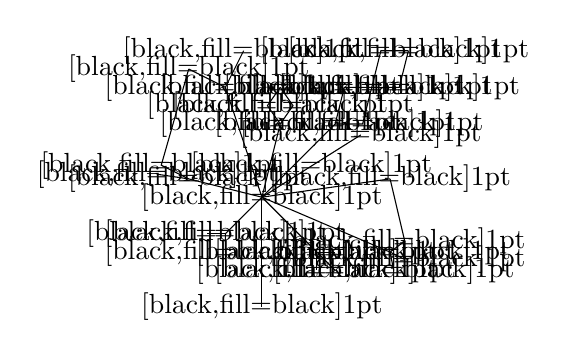
\begin{tikzpicture}[scale=0.465]
\draw (0,0) node {\tikzcircle[black,fill=black]{1pt}} -- (-1,3)  node {\tikzcircle[black,fill=black]{1pt}} -- (-2,3.5) node {\tikzcircle[black,fill=black]{1pt}};
%\draw (-1,3) -- (-2,3.5);
\draw (-1,3) -- (-0.5,4) node {\tikzcircle[black,fill=black]{1pt}};
\draw (0,0) -- (0.5,2) node {\tikzcircle[black,fill=black]{1pt}} -- (0.15,2.5) node {\tikzcircle[black,fill=black]{1pt}} -- (0.5,3) node {\tikzcircle[black,fill=black]{1pt}};
\draw (0.5,2) -- (0.85,2.5) node {\tikzcircle[black,fill=black]{1pt}} -- (0.5,3); 
\draw (0,0) -- (2,2) node {\tikzcircle[black,fill=black]{1pt}} -- (2.25,3) node {\tikzcircle[black,fill=black]{1pt}} -- (3,3) node {\tikzcircle[black,fill=black]{1pt}} -- (3.25,4) node {\tikzcircle[black,fill=black]{1pt}} -- (4,4) node {\tikzcircle[black,fill=black]{1pt}};
\draw          (2,2) -- (2.75,2) node {\tikzcircle[black,fill=black]{1pt}} -- (3,3) -- (3.75,3) node {\tikzcircle[black,fill=black]{1pt}} -- (4,4);
\draw (0,0) -- (1.35,0.85) node {\tikzcircle[black,fill=black]{1pt}} -- (2.7,1.7) node {\tikzcircle[black,fill=black]{1pt}};
\draw (0,0) -- (3.5,0.5) node {\tikzcircle[black,fill=black]{1pt}};
\draw (0,0) -- (3.5,-1.5) node {\tikzcircle[black,fill=black]{1pt}} -- (3.9,-1.2) node {\tikzcircle[black,fill=black]{1pt}} -- (3.5,0.5);
\draw (3.5,-1.5) -- (3.9,-1.7) node {\tikzcircle[black,fill=black]{1pt}};
\draw (3.5,-1.5) -- (3.6,-2) node {\tikzcircle[black,fill=black]{1pt}};
\draw (0,0) -- (1.5,-1.5) node {\tikzcircle[black,fill=black]{1pt}} -- (2,-2) node {\tikzcircle[black,fill=black]{1pt}};
\draw (1.5,-1.5) -- (2,-1.5) node {\tikzcircle[black,fill=black]{1pt}};
\draw (1.5,-1.5) -- (1.5,-2) node {\tikzcircle[black,fill=black]{1pt}};
\draw (0,0) -- (0,-3) node {\tikzcircle[black,fill=black]{1pt}};
\draw (0,0) -- (-1,-1) node {\tikzcircle[black,fill=black]{1pt}} -- (-1,-1.5) node {\tikzcircle[black,fill=black]{1pt}};
\draw (-1,-1) -- (-1.5,-1) node {\tikzcircle[black,fill=black]{1pt}};
\draw (0,0) -- (-2,0.5) node {\tikzcircle[black,fill=black]{1pt}} -- (-2.85,0.625) node {\tikzcircle[black,fill=black]{1pt}};
\draw  (-2,0.5) -- (-2.75,0.875) node {\tikzcircle[black,fill=black]{1pt}} -- (-2,3.5);
\end{tikzpicture}}
	& \framebox{\begin{tikzpicture}[scale=0.5]
  \star{0}{2.5};
  \star{-2}{0};
  \star{-0.5}{-2};
  \draw (-2,0) -- (0,0.5) -- (0,2.5);
  \draw (-0.5,-2) -- (0,0.5) node {\tikzcircle[black,fill=black]{1pt}} -- (2,0) node {\tikzcircle[black,fill=black]{1pt}} -- (4,0.75) node {\tikzcircle[black,fill=black]{1pt}} -- (3.5,2.75);
  \draw (4,0.75) -- (6,-0.5);
  \star{3.5}{2.75};
  \star{6}{-0.5};
\end{tikzpicture}}
	& \framebox{
	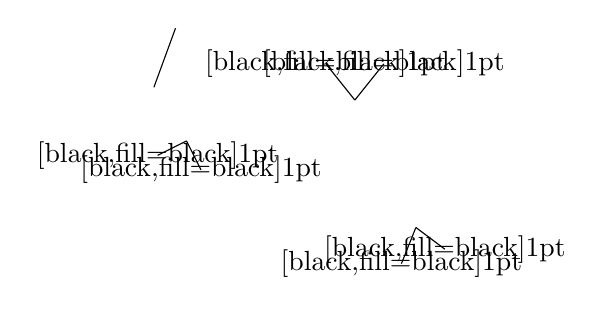
\begin{tikzpicture}[scale=0.92]
  \starseven{-1.5}{0.5}{0};
  \starseven{0.5}{-0.75}{20};
  \draw ({0.5+cos(82.8+20)},{-0.75+sin(82.8+20)}) -- ({0.5+cos(82.8+20)+0.4},{-0.75+sin(82.8+20)+0.5}) node {\tikzcircle[black,fill=black]{1pt}};
  \draw ({0.5+cos(82.8+20)},{-0.75+sin(82.8+20)}) -- ({0.5+cos(82.8+20)-0.4},{-0.75+sin(82.8+20)+0.5}) node {\tikzcircle[black,fill=black]{1pt}};
  \draw ({0.5+cos(288.4+20)},{-0.75+sin(288.4+20)}) -- ({0.5+cos(288.4+20)-0.2},{-0.75+sin(288.4+20)-0.5}) node {\tikzcircle[black,fill=black]{1pt}};
  \draw ({0.5+cos(288.4+20)},{-0.75+sin(288.4+20)}) -- ({0.5+cos(288.4+20)+0.4},{-0.75+sin(288.4+20)-0.3}) node {\tikzcircle[black,fill=black]{1pt}};
%  \draw ({0.5+cos(288.4+20)},{-0.75+sin(288.4+20)}) -- ({0.5+cos(237+20)},{-0.75+sin(237+20)});
  \draw ({-1.5+cos(134.2)},{0.5+sin(134.2)}) -- ({-1.5+cos(185.6)},{0.5+sin(185.6)});
  \draw ({-1.5+cos(237)},{0.5+sin(237)}) -- ({-1.5+cos(237)+0.2},{0.5+sin(237)-0.4}) node {\tikzcircle[black,fill=black]{1pt}};
  \draw ({-1.5+cos(237)},{0.5+sin(237)}) -- ({-1.5+cos(237)-0.4},{0.5+sin(237)-0.2}) node {\tikzcircle[black,fill=black]{1pt}};
\end{tikzpicture}}
\\
$g_1$ & $g_2$ & $g_3$
\end{tabular}
\end{center}


%\vfill
%
%\emph{Further Investigation.}
%\begin{enumerate}[label=\emph{\arabic*.}]
%\item Can you think of other forms for $H(P,t)$? 
%
%\item If, instead of a logistic model, you include an extinction threshold as well, what can you say about the model for constant effort fishing? for constant rate fishing? Is it a useful addition to the model? Have fun with it!
%\end{enumerate}



\vfill

\begin{graybox}
Based on ``How to measure influence and impact'', ICM 2014.
\end{graybox}


\begin{graybox}
\hfill ``\erdostitle'' is a collaboration with Yvan Saint-Aubin.	
\end{graybox}


\begin{noexercises}
\end{noexercises}
